\begin{figure}
    \centering
    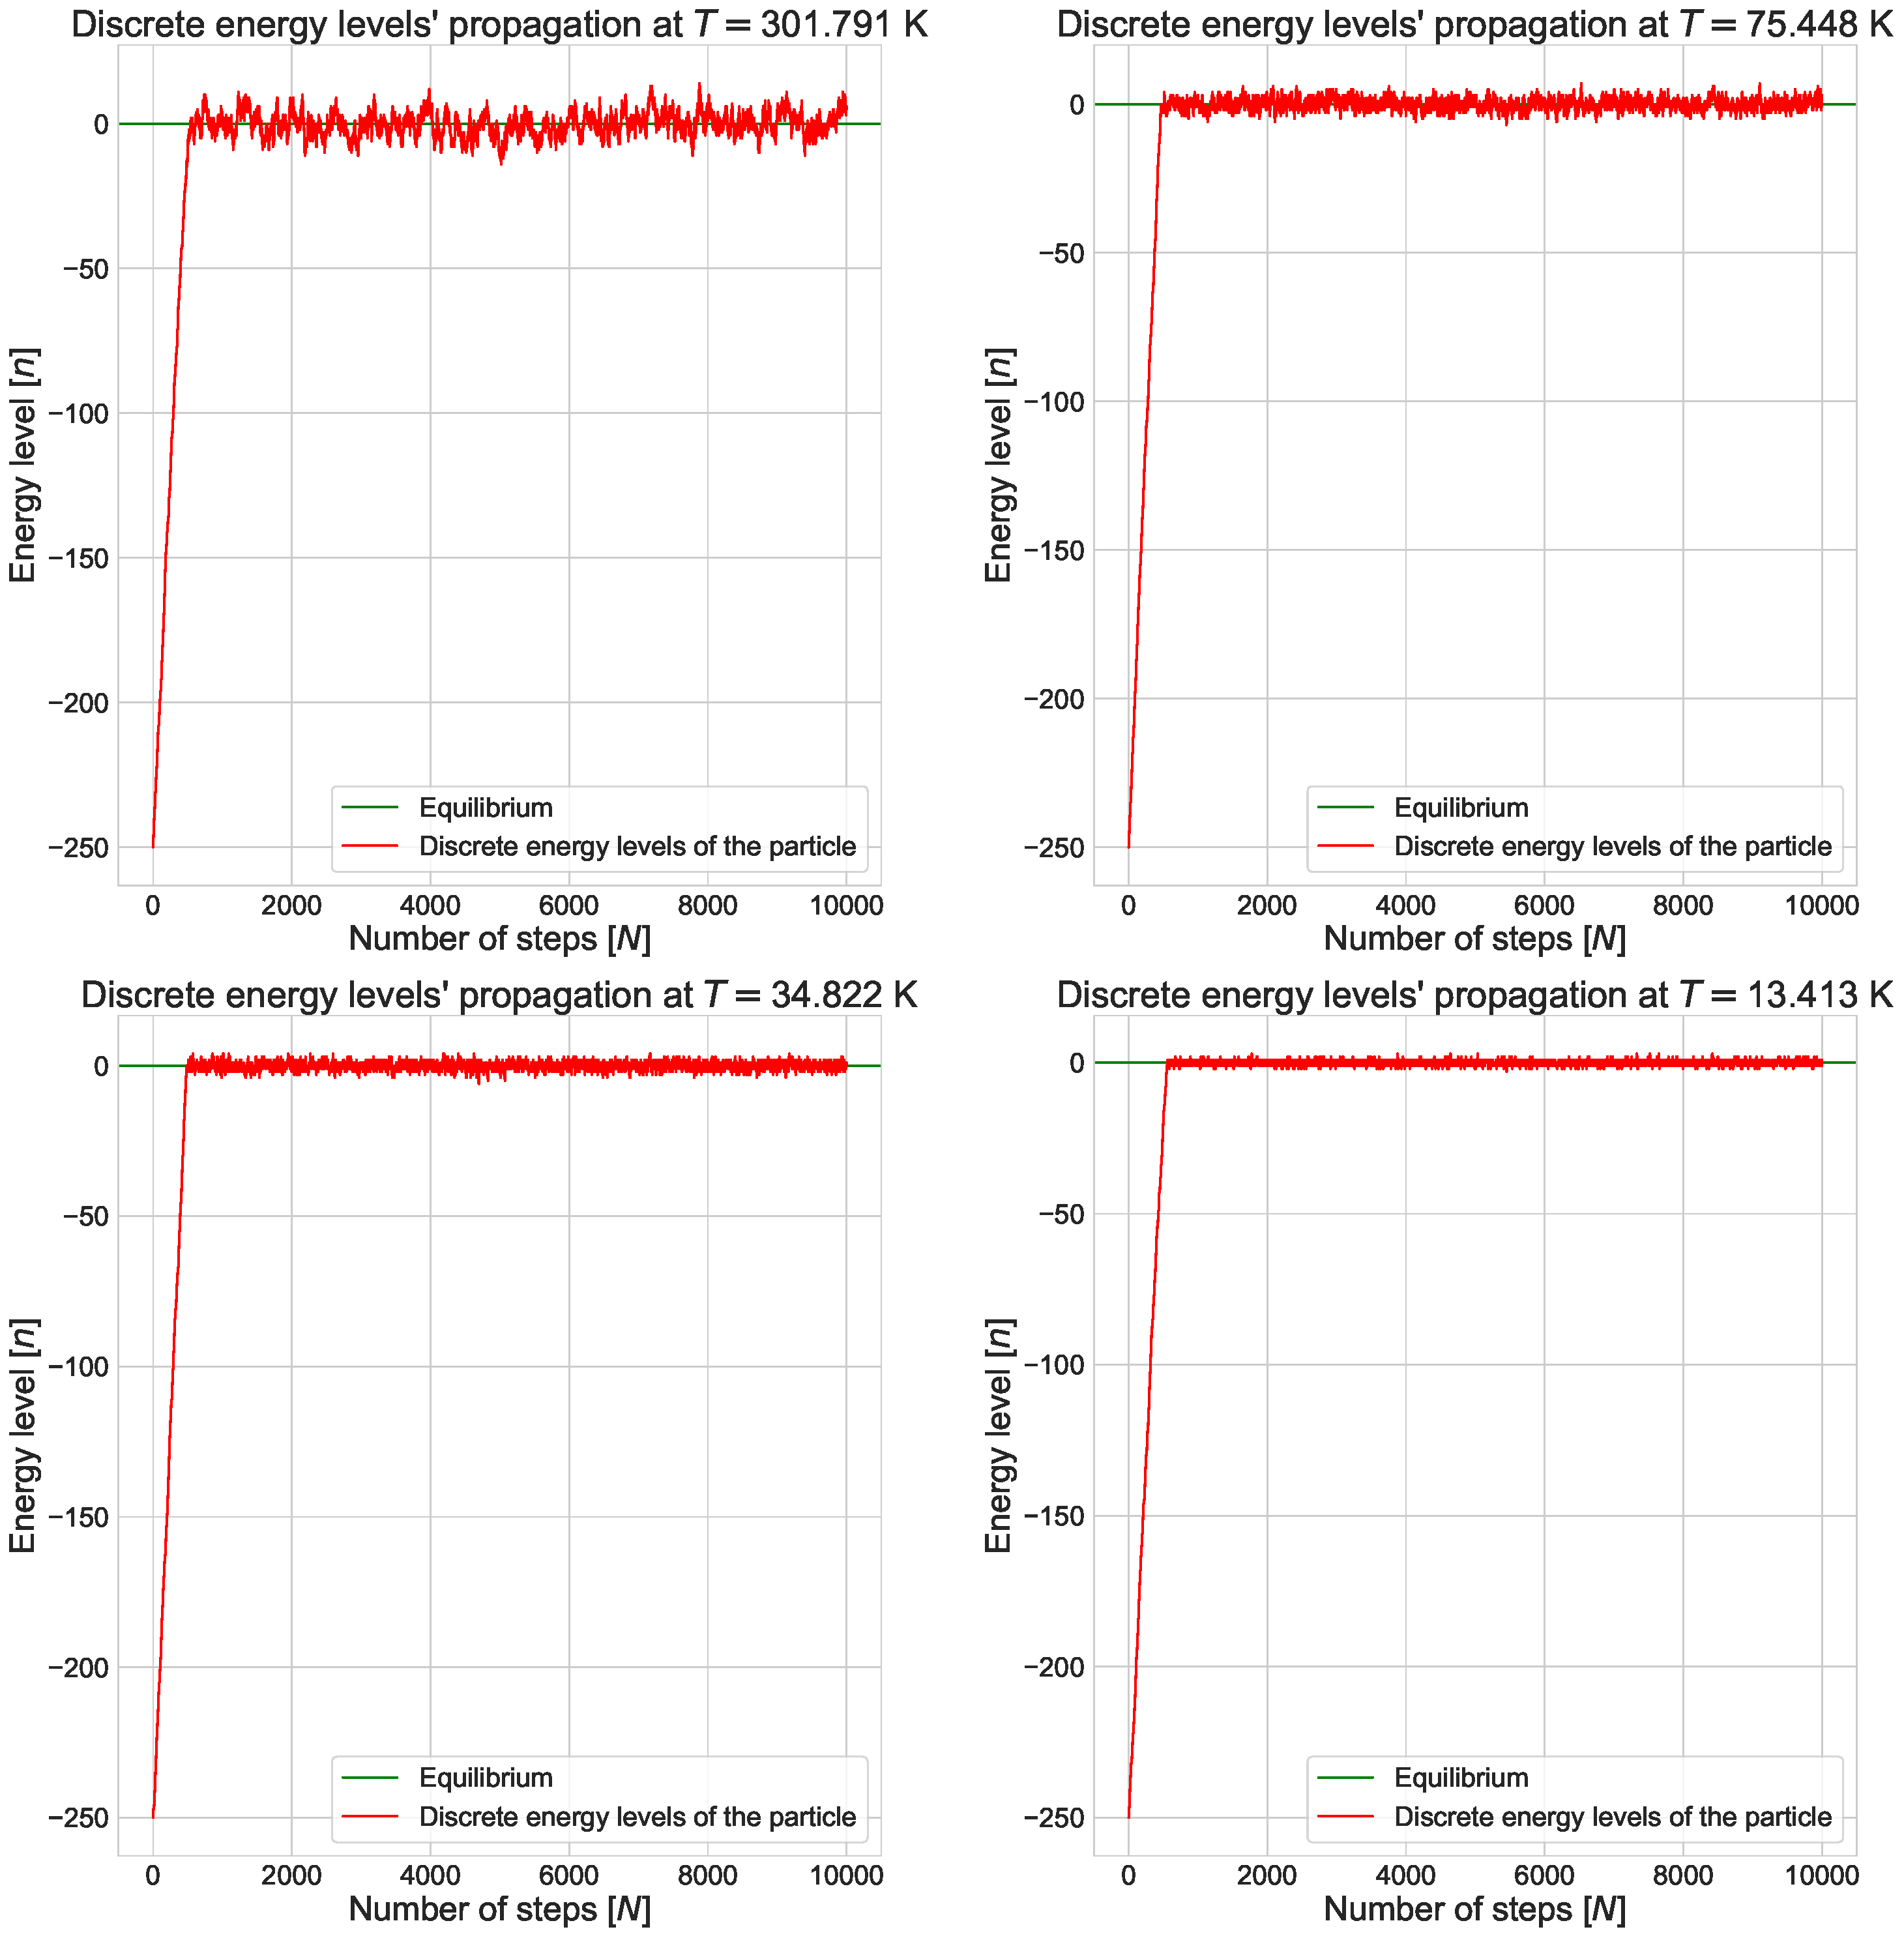
\includegraphics[width=\textwidth]{images/discrete_levels.pdf}
    \caption{The particle's jumps between discrete energy levels respect to time}
    \label{fig:fig1}
\end{figure}

\begin{figure}
    \centering
    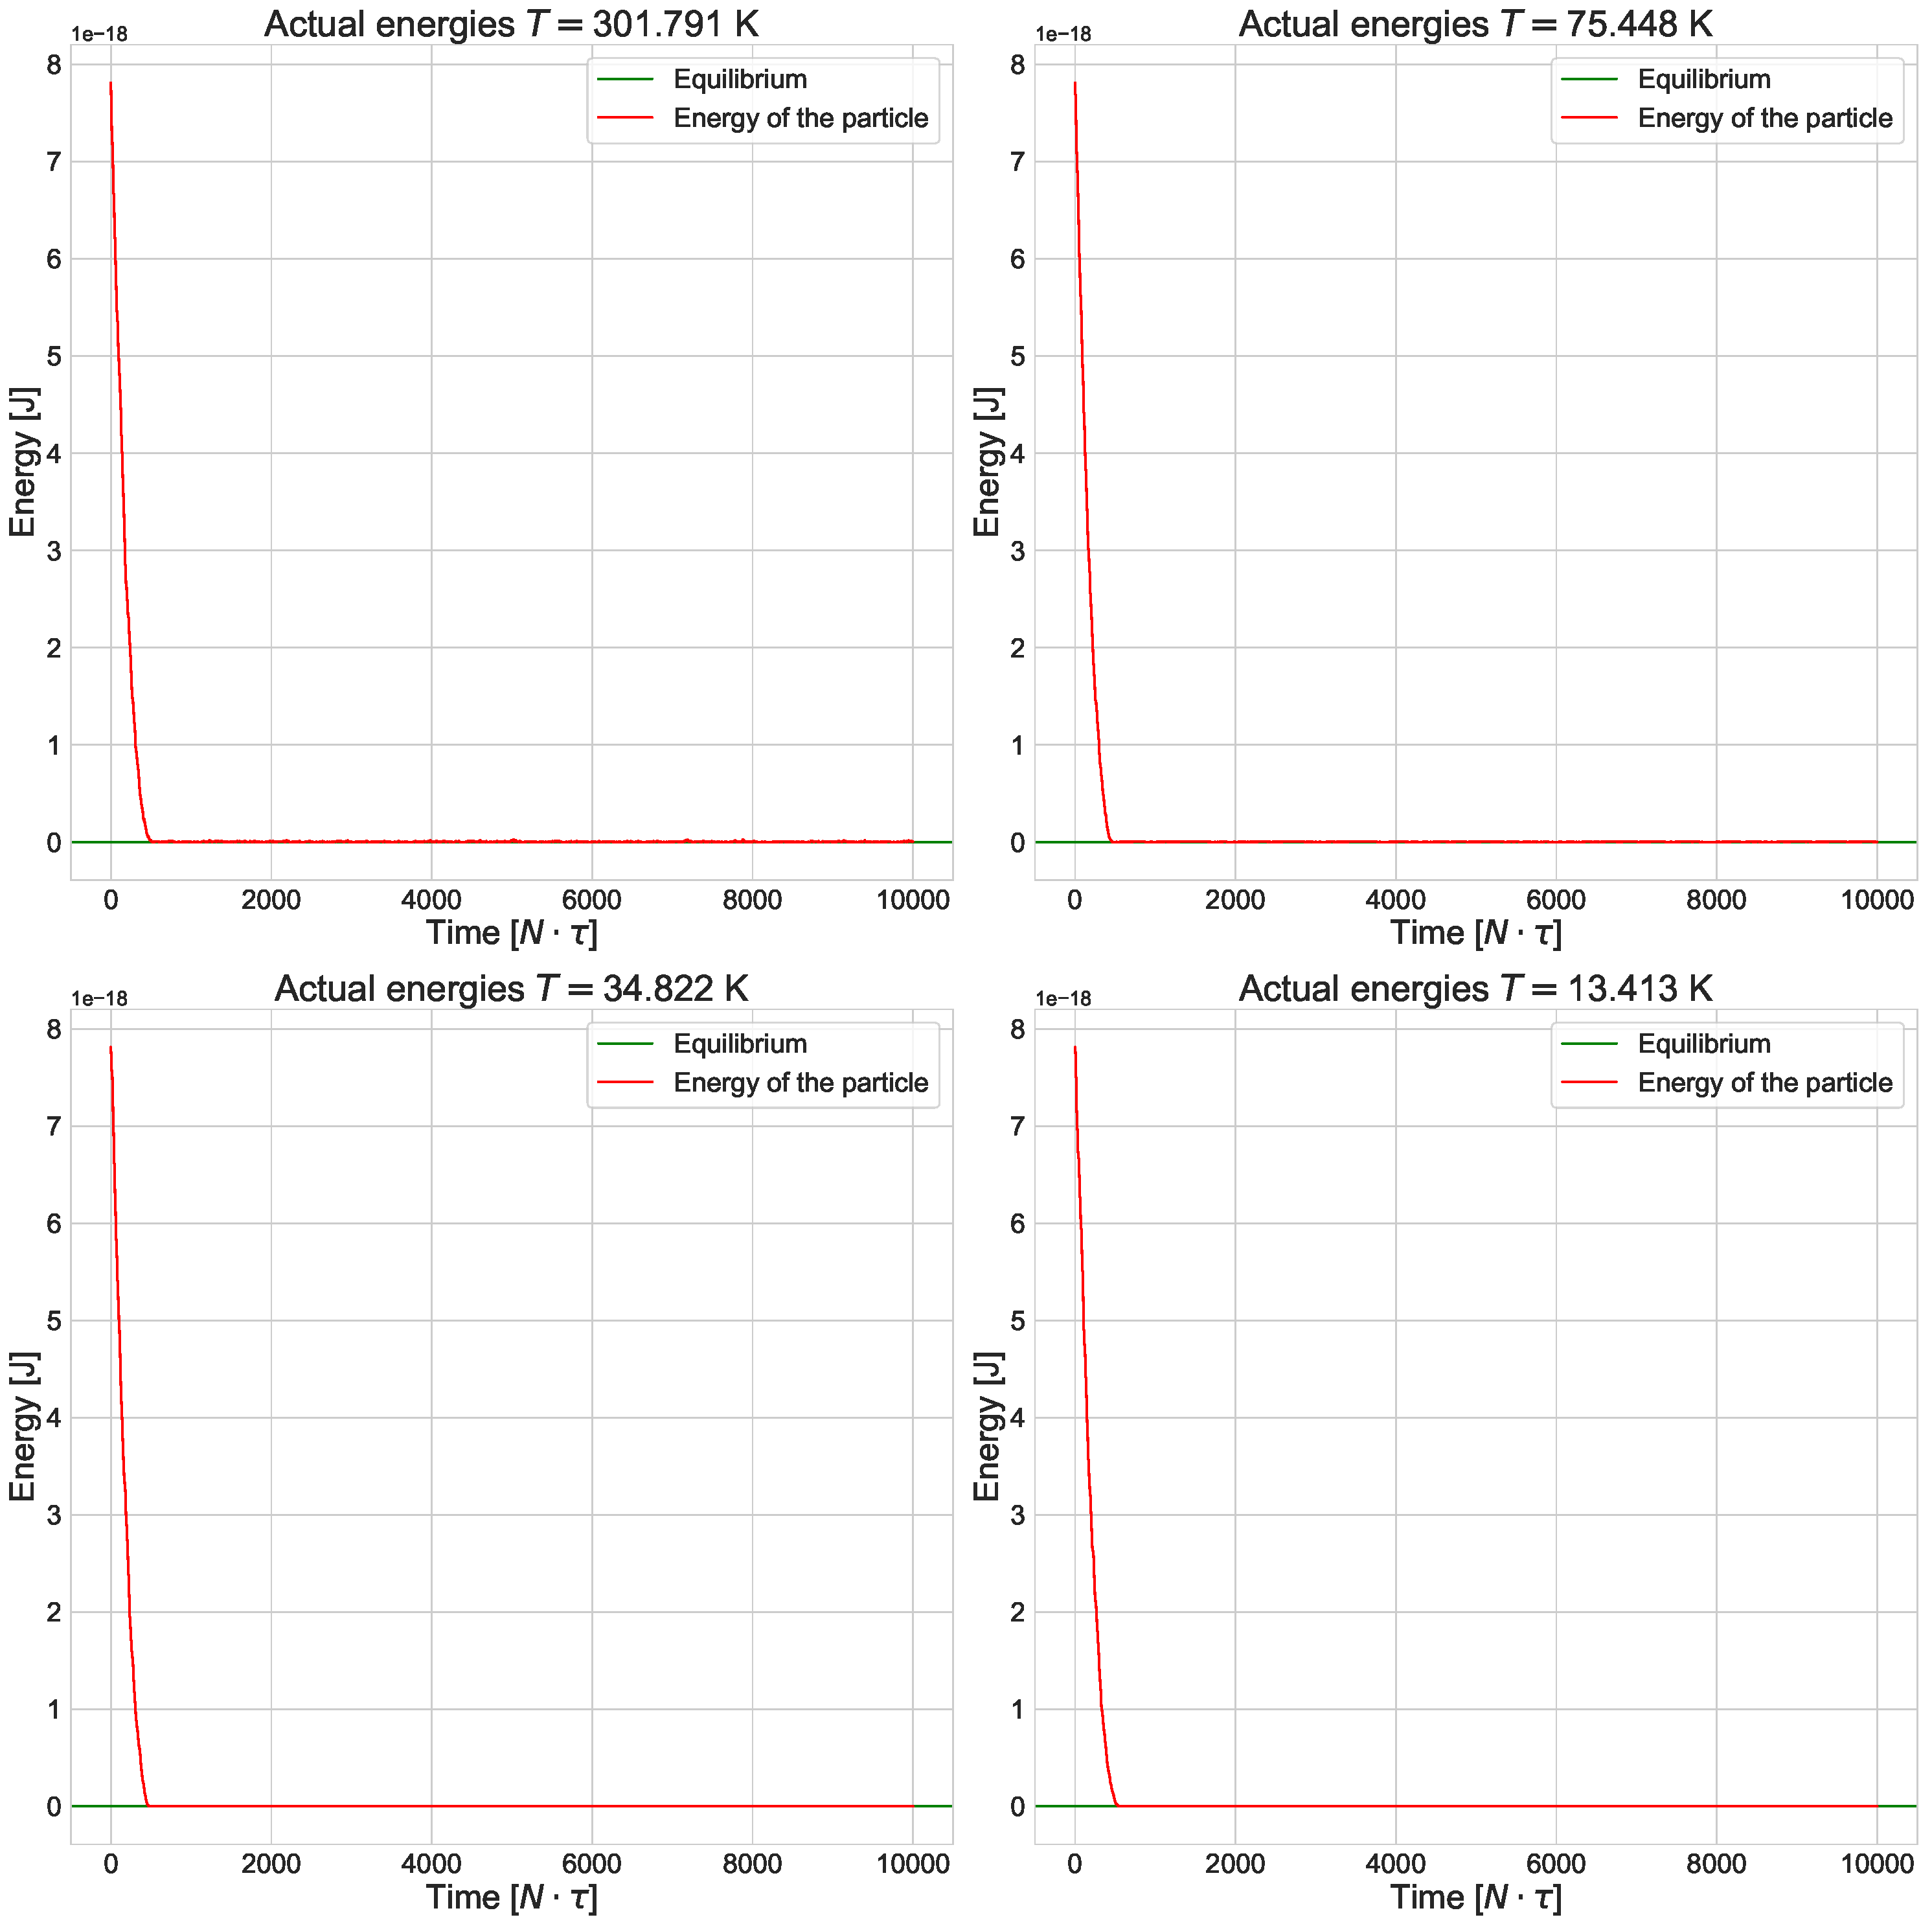
\includegraphics[width=\textwidth]{images/discrete_energies.pdf}
    \caption{Changes in the actual energies during the particle's propagation}
    \label{fig:fig2}
\end{figure}

\begin{figure}
    \centering
    \includegraphics[width=\textwidth]{images/discrete_levels_various_start.pdf}
    \caption{The particle's jumps between discrete energy levels respect to time for 25 different $x \left( t = 0 \right)$ starting points}
    \label{fig:fig3}
\end{figure}

\begin{figure}
    \centering
    \includegraphics[width=\textwidth]{images/discrete_energies_various_start.pdf}
    \caption{Changes in the actual energies during the particle's propagation for 25 different $x \left( t = 0 \right)$ starting points}
    \label{fig:fig4}
\end{figure}

\begin{figure}
    \centering
    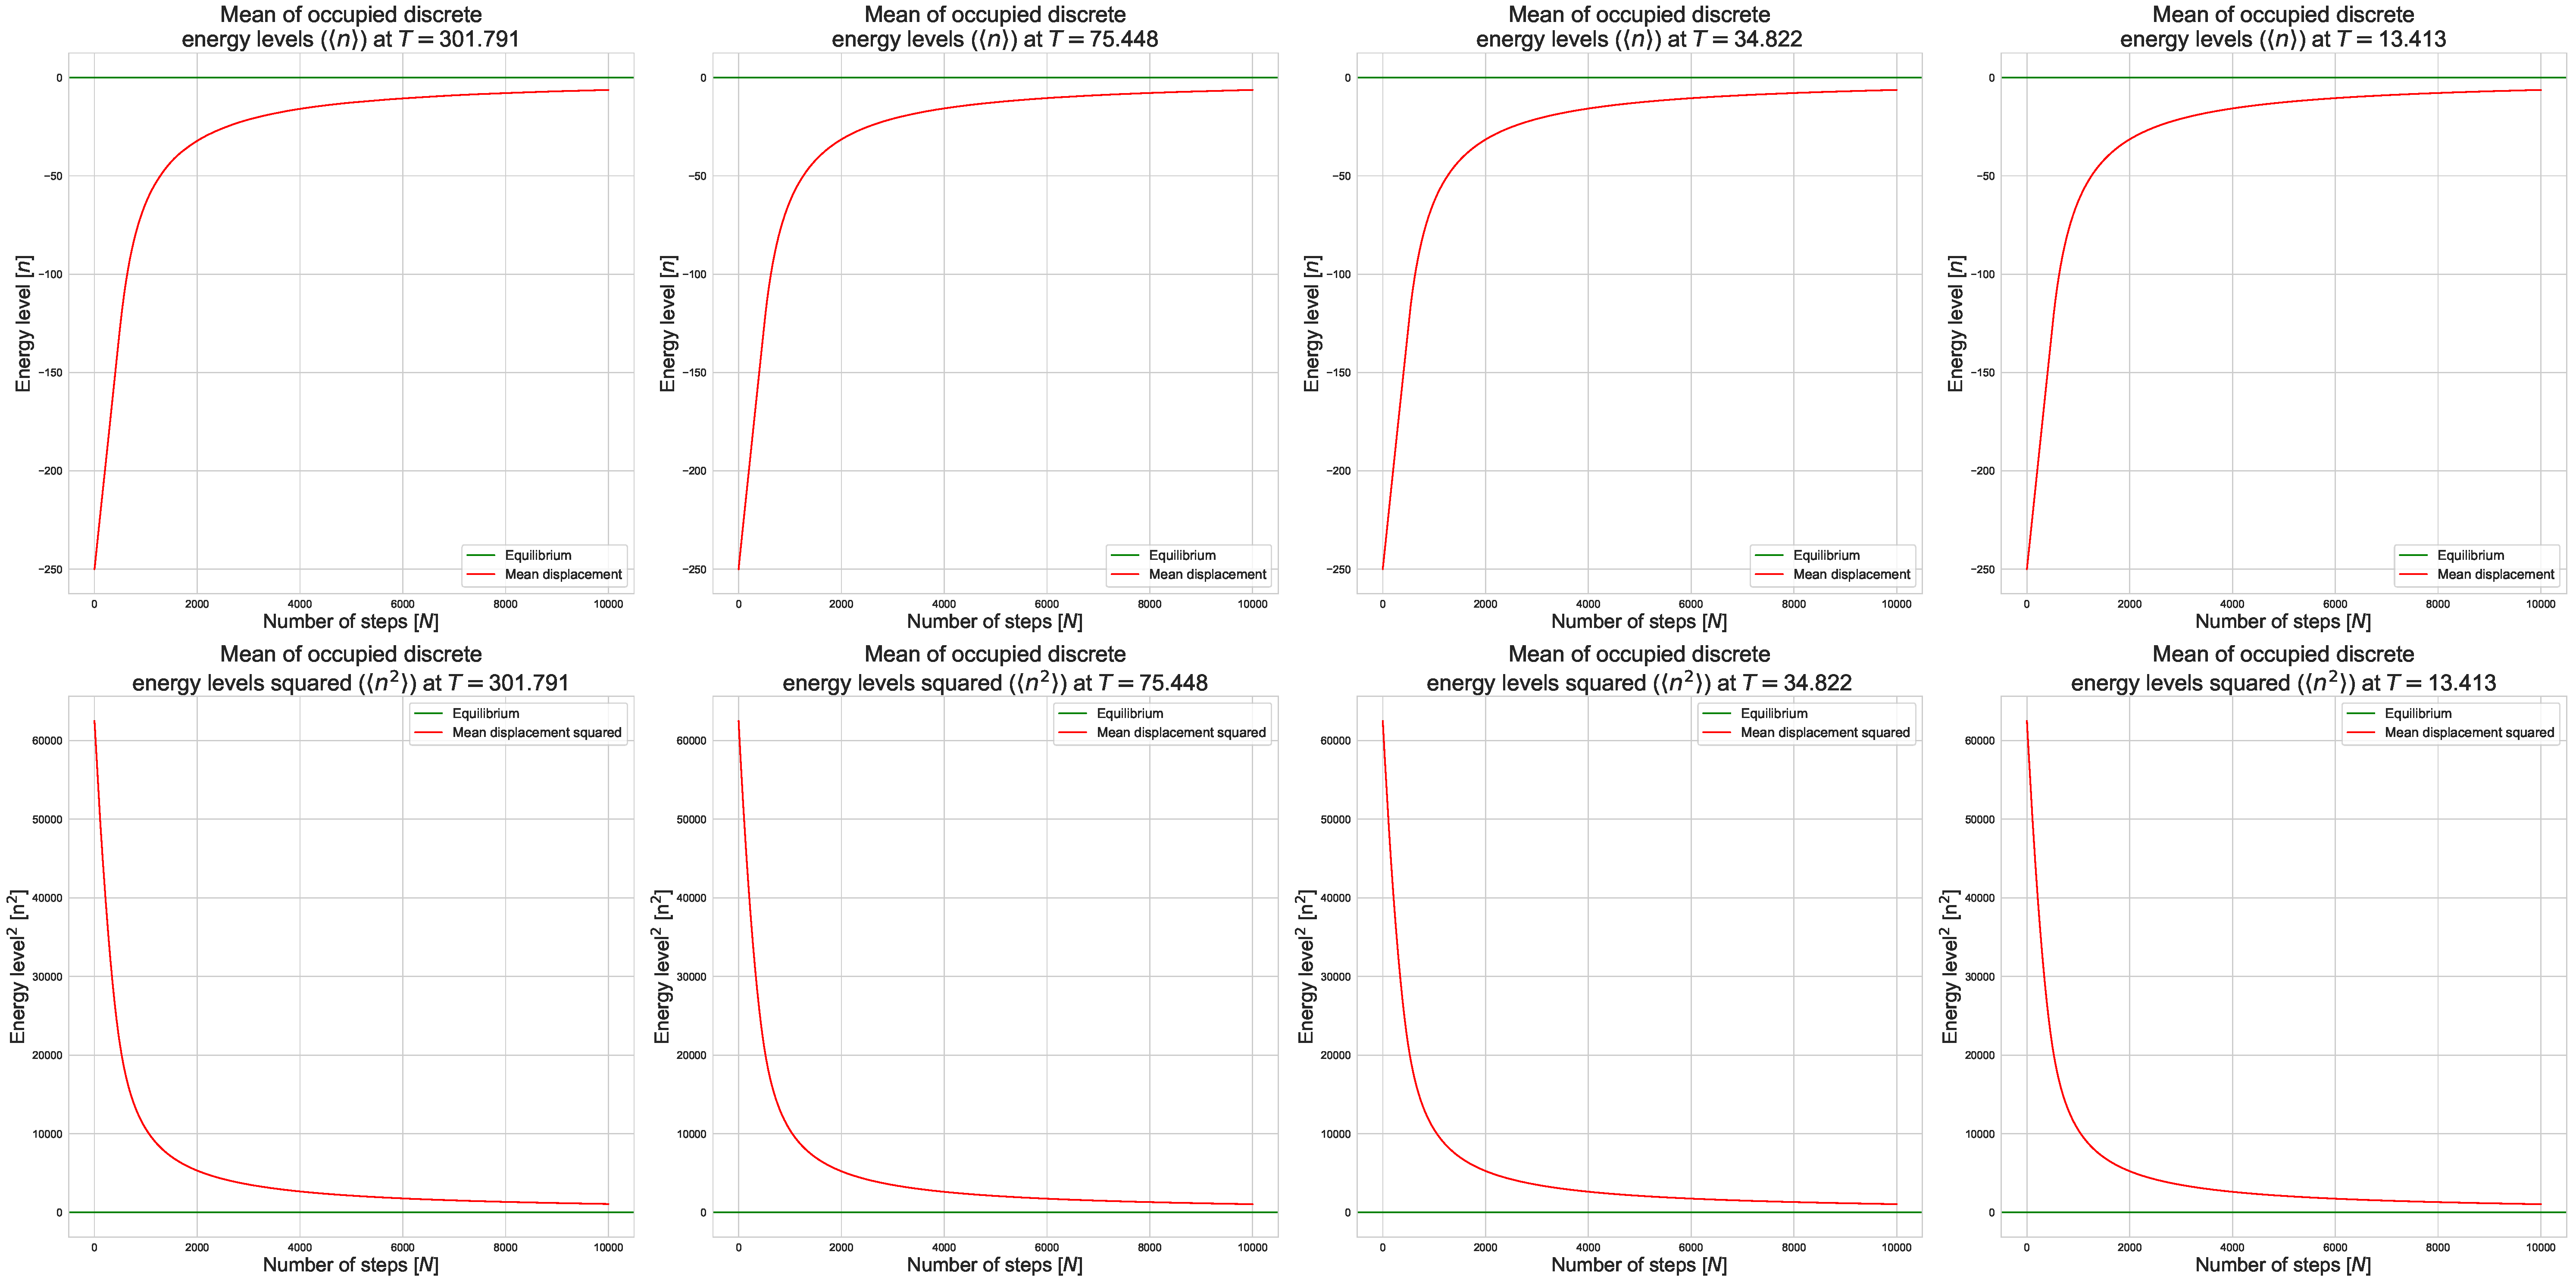
\includegraphics[width=\textwidth]{images/discrete_levels_expected.pdf}
    \caption{Mean of the indeces of the occupied energy levels, when the particle starts its propagation from the $x = -250$ point}
    \label{fig:fig5}
\end{figure}

\begin{figure}
    \centering
    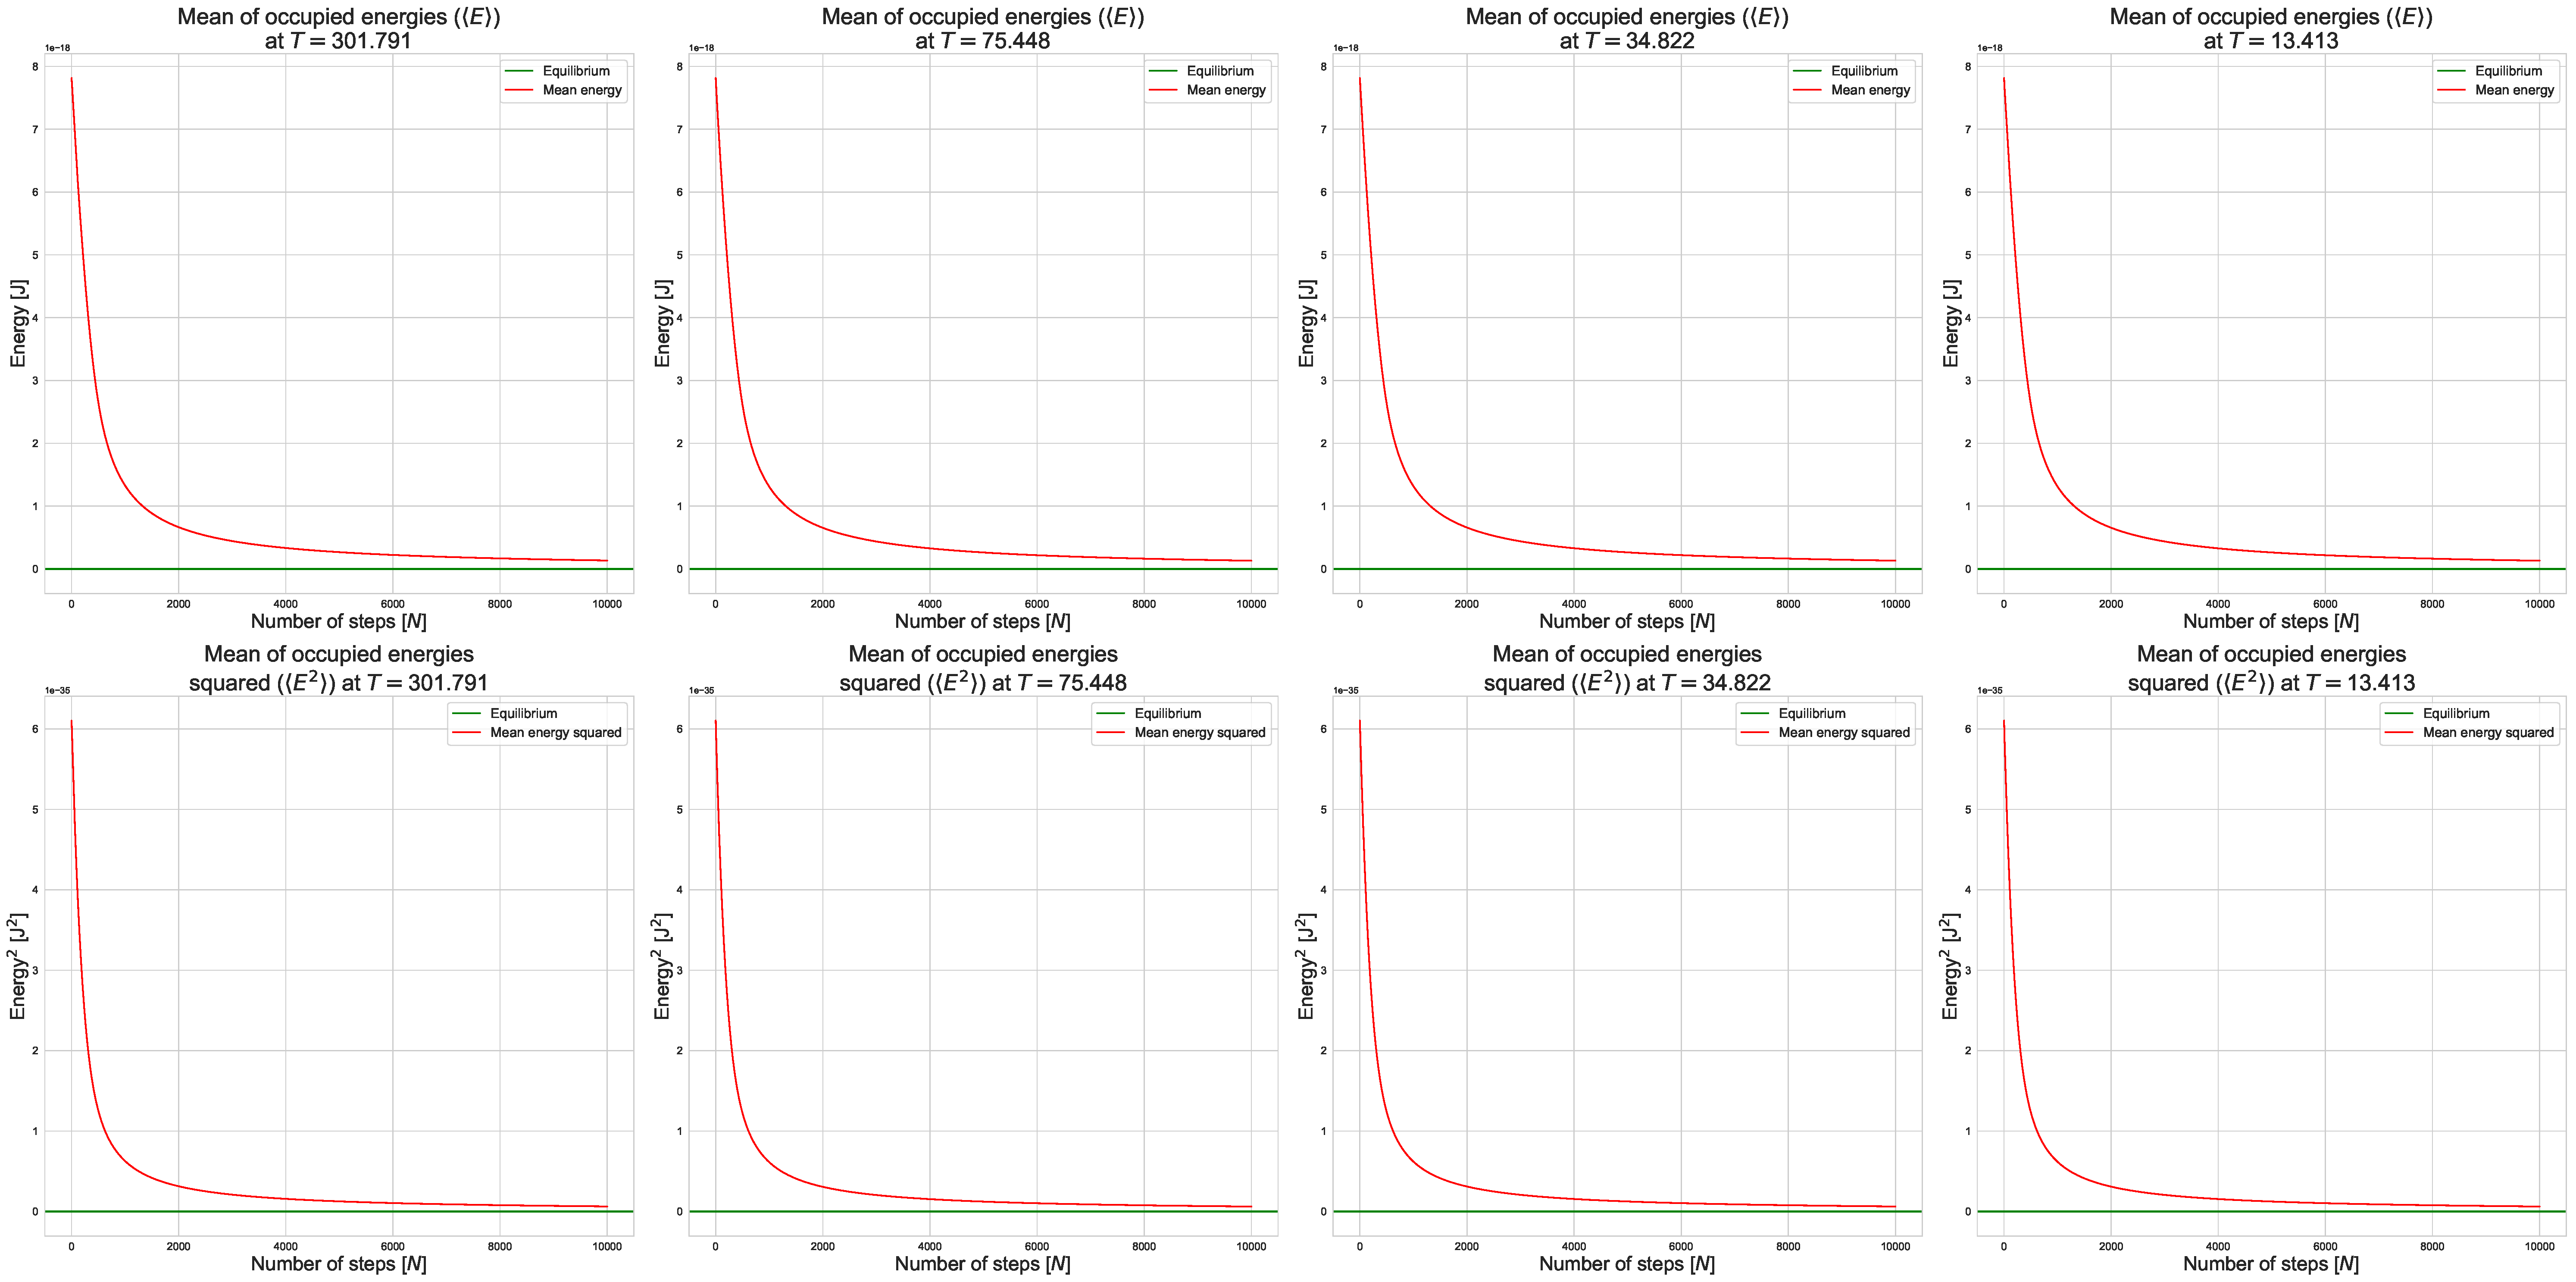
\includegraphics[width=\textwidth]{images/discrete_energies_expected.pdf}
    \caption{Mean of the occupied energies, when the particle starts its propagation from the $x \left( t = 0 \right) = -250$ point}
    \label{fig:fig6}
\end{figure}

\begin{figure}
    \centering
    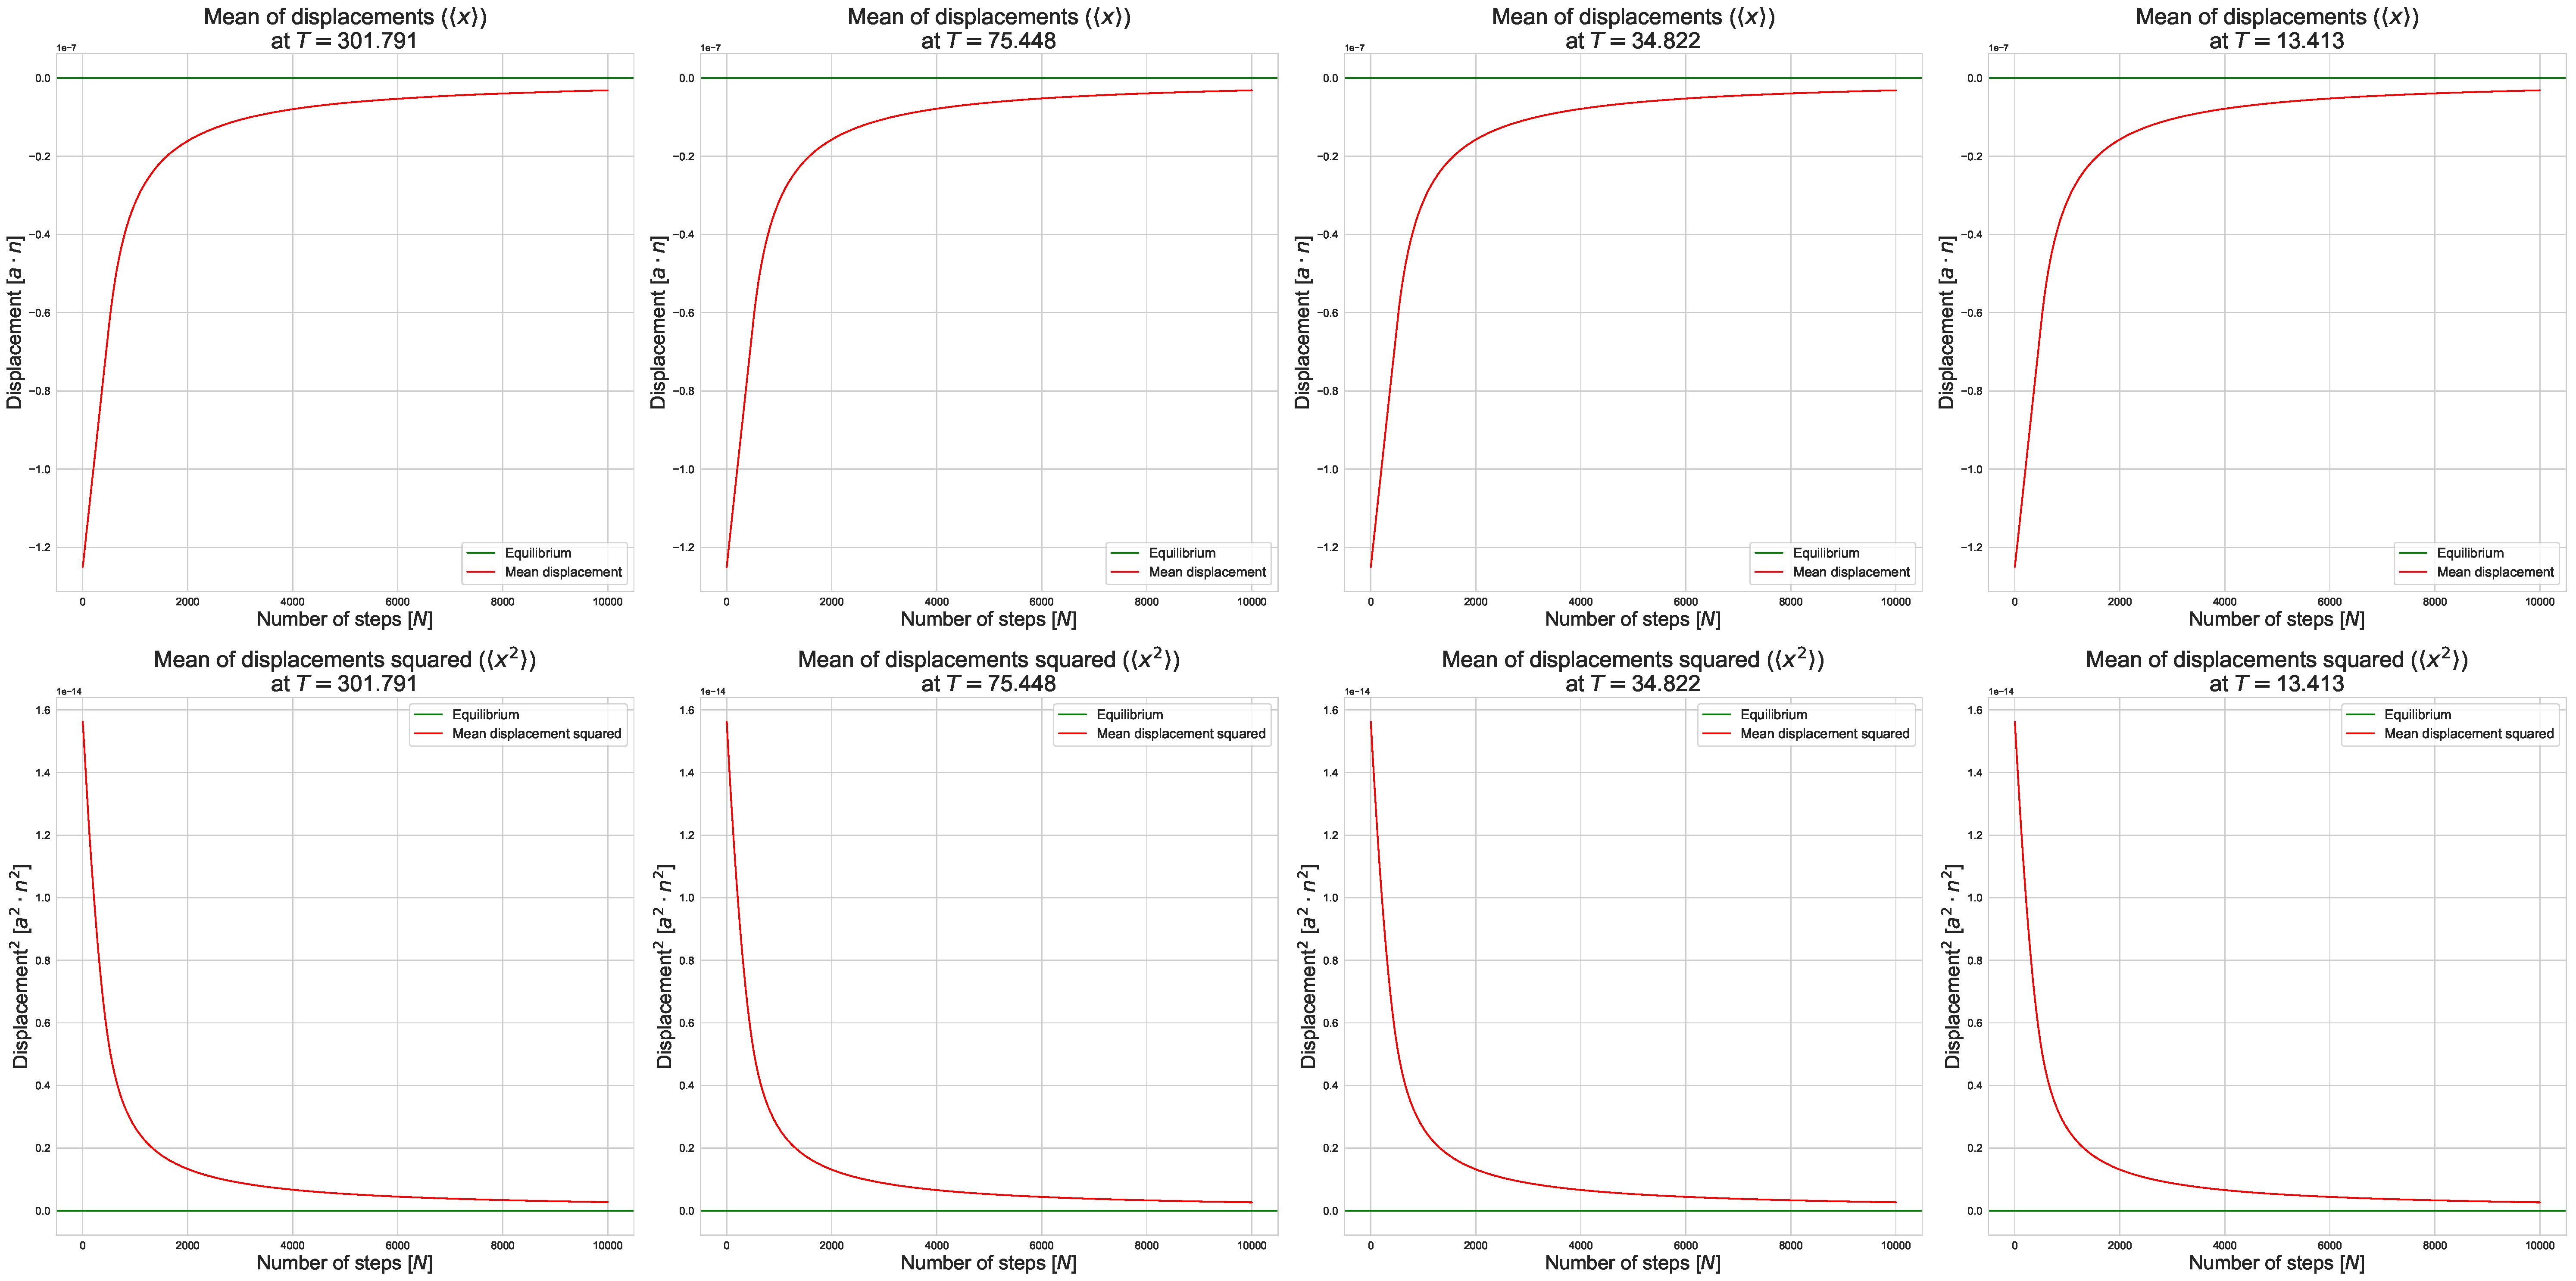
\includegraphics[width=\textwidth]{images/discrete_displacements_expected.pdf}
    \caption{Mean of the distances of the particle from the $x = 0$ grid point, when the particle starts its propagation from the $x \left( t = 0 \right) = -250$ point}
    \label{fig:fig7}
\end{figure}

\begin{figure}
    \centering
    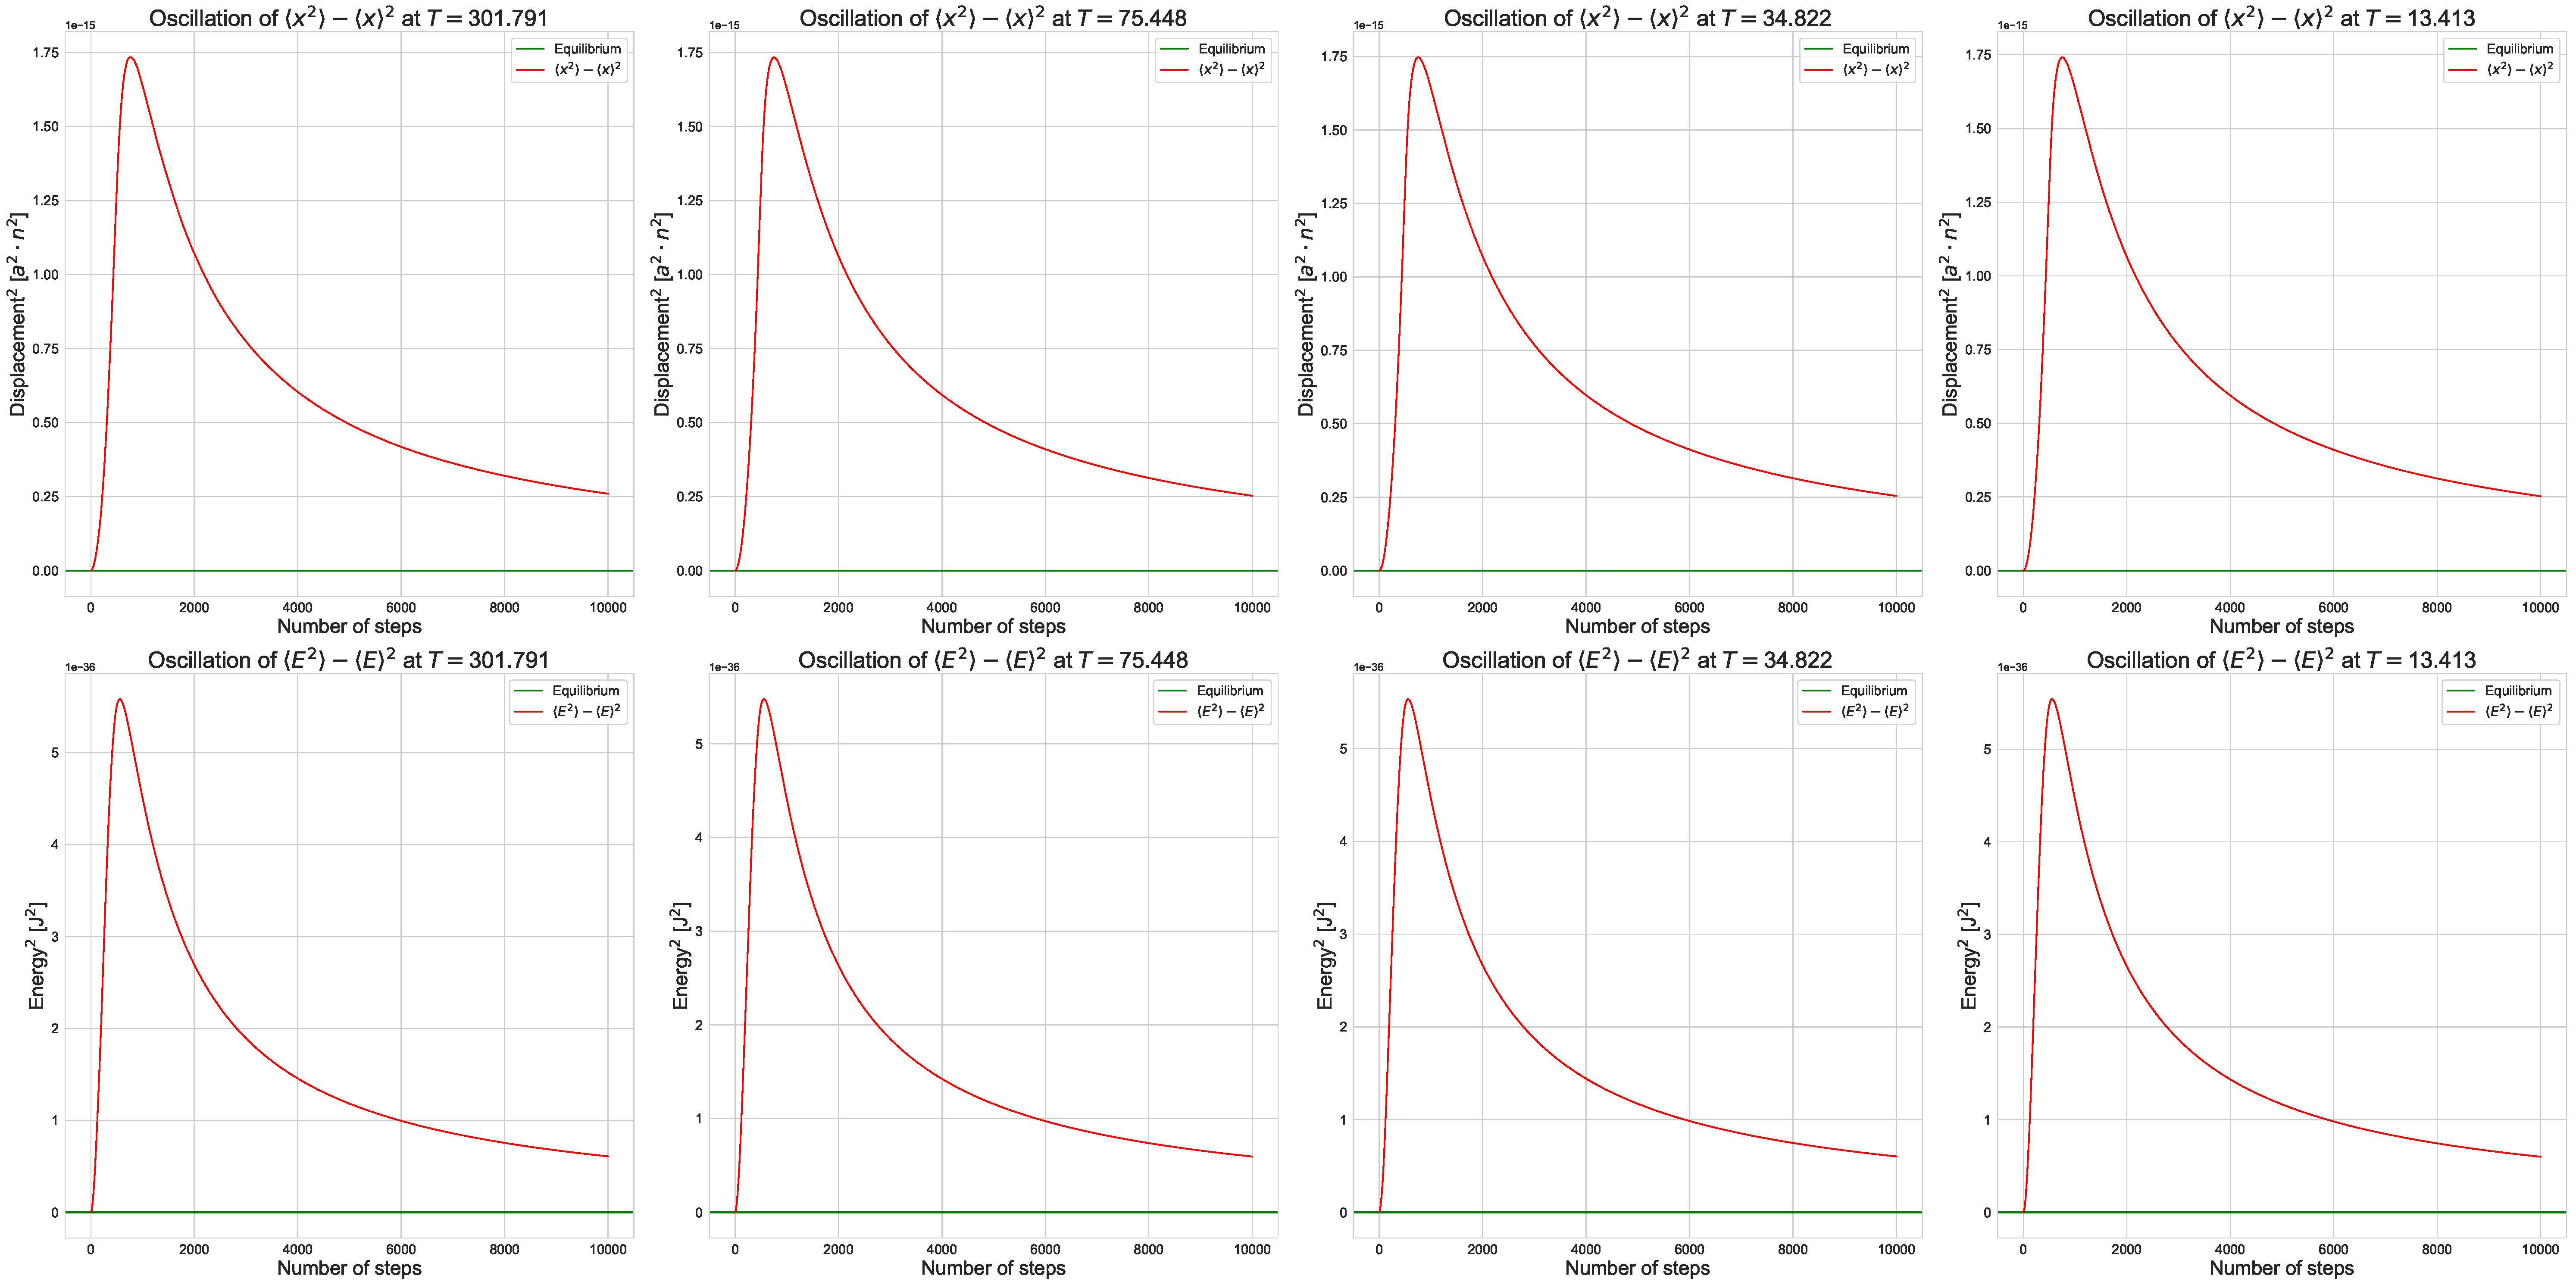
\includegraphics[width=\textwidth]{images/oscillation.pdf}
    \caption{Oscillation of $\left< x^{2} \right> - \left< x \right>^{2}$ and $\left< E^{2} \right> - \left< E \right>^{2}$, when the particle starts its propagation from the $x \left( t = 0 \right) = -250$ point}
    \label{fig:fig8}
\end{figure}